\documentclass[a4paper]{article}

\usepackage[utf8]{inputenc}
\usepackage[serbian]{babel}

\usepackage{tikz}
\usepackage{tcolorbox}
\usepackage{amsmath}
\usepackage{amsthm}
\usepackage{nameref}
\usepackage{listings}
\usepackage{fancyhdr}

\makeatletter
\newcommand*{\currentname}{\@currentlabelname}
\makeatother

\begin{document}
    \begin{titlepage}
    \begin{tabular}{ l  c   r  }
        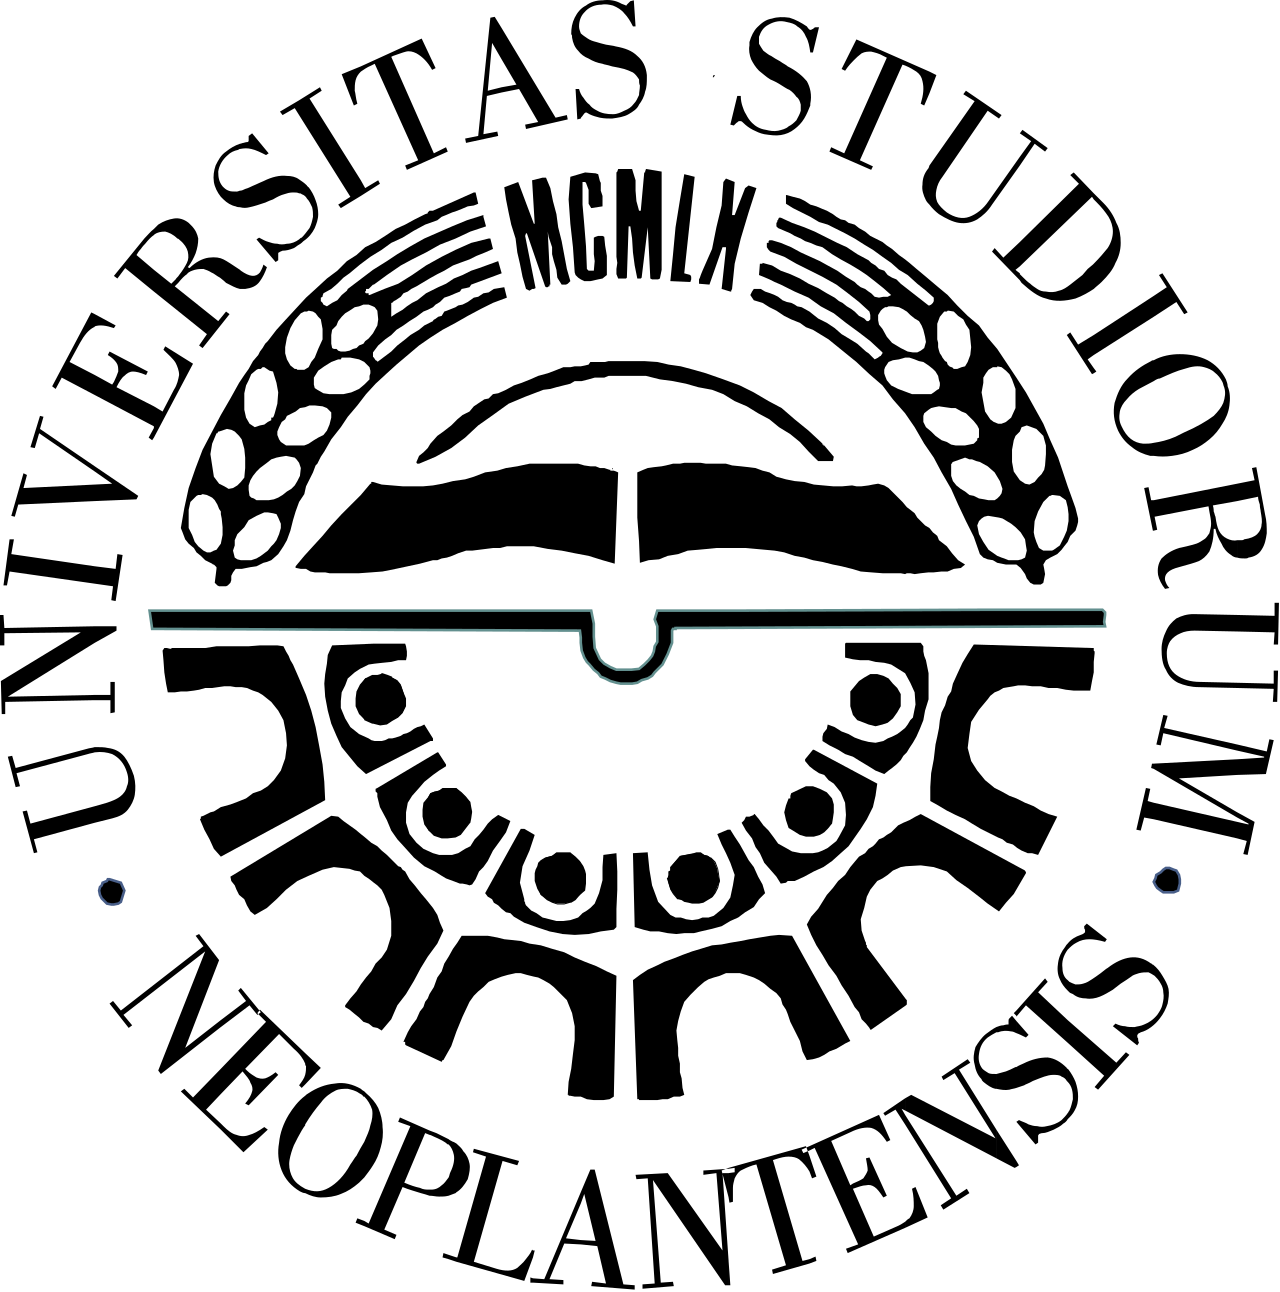
\includegraphics[height=0.1\textwidth, width=0.1\textwidth]{img/uns.png} &
        \begin{tabular}{c}
            \large\textbf{UNIVERZITET U NOVOM SADU} \\
            \large\textbf{FAKULTET TEHNIČKIH NAUKA}  \\
        \end{tabular}
        
\includegraphics[height=0.1\textwidth, width=0.1\textwidth]{img/ftn-logo.jpg}
    \end{tabular}
    \vspace*{1cm}
    \begin{flushleft}
        UNIVERZITET U NOVOM SADU \\
        FAKULTET TEHNIČKIH NAUKA \\
        NOVI SAD \\
        Departman za računarstvo i automatiku \\
        Odsek za računarsku tehniku i računarske komunikacije \\
    \end{flushleft}
    \vspace*{2cm}
    \begin{center}
        \LARGE\textbf{ISPITNI RAD}
    \end{center}
    \vspace*{0.25cm}
    \begin{flushleft}
        \begin{tabular}{l l}
            Kandidat:& Lazar Nagulov \\
            Broj indeksa:& SV61/2022 \\
            & \\
            Predmet:&    Objektno orijentisano programiranje 2 \\
            Tema rada:&	Sudoku \\
            & \\
            & \\
            Mentor rada:&    dr Miodrag Đukić
        \end{tabular}
    \end{flushleft}
    \vfill
    \begin{center}
        Novi Sad, decembar, 2023.
    \end{center}
\end{titlepage}
    \pagestyle{fancy}
    
\rhead{SADRŽAJ}
\lhead{}
\pagenumbering{Roman}
\tableofcontents
\newpage

\rhead{SPISAK SLIKA}
\listoffigures
\newpage

\rhead{SPISAK TABELA}
\listoftables
\newpage
    
    \section{Uvod}
    \pagenumbering{arabic}
    \rhead{1. Uvod}
    \subsection{Sudoku}
    Sudoku je logička zagonetka najčešće u obliku $9 \times 9$ tabele (matrice).
    U prazna polja tabele se upisuju cifre, tako da se svaka cifra mora pojaviti
    tačno jednom u svakom redu, svakoj koloni i svakoj $3\times 3$ podmatrici (bloku).
    \begin{figure}[h]
        \centering
        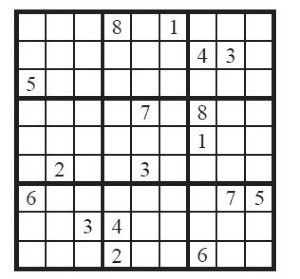
\includegraphics[width=0.5\textwidth, height=0.5\textwidth]{img/sudoku-example.jpg}
        \caption{Primer sudoku zagonetke}
    \end{figure}
    \par Zagonetka ne mora da ima jedno rešenje, ali je standard da ga ima. Primer rešenje zagonetke sa slike 1:
    \begin{figure}[h]
        \centering
        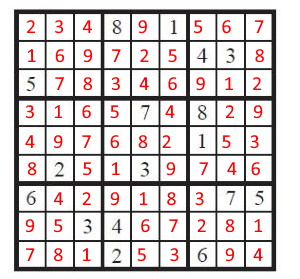
\includegraphics[width=0.5\textwidth, height=0.5\textwidth]{img/sudoku-example-sol.jpg}
        \caption{Primer rešenja sudoku zagonetke}
    \end{figure}
    
    \subsection{Zadatak}
    Realizovati konzolnu aplikaciju koja omogućava rešavanje i generisanje sudoku zagonetki.    
    \newpage

    \rhead{3. Algoritmi za rešavanje zagonetke}
    \section{Algoritmi za rešavanje zagonetke}
    
    \subsection{Obrnuta pretraga}
    Najtrivijalniji algoritam za rešavanje sudoku zagonetke je obrnuta pretraga (eng. Backtracking).
    Ovo je algoritam grube sile (eng. Brute force) koji isprobava sve moguće kombinacije. Dakle, potrebno je da se prođe kroz
    svako polje u tabeli. Ukoliko je polje prazno, upisujemo cifru koja u trenutnoj tabeli ispunjava sva pravila. Nakon upisivanje cifre, rekurzivno pozivamo funkciju 
    - pokušavamo da pronađe rešenje sa novom tabelom. Ukoliko rešenje nije pronađeno, vraćamo se nazad i upisujemo drugu cifru. 
    \par Vremenska složenost ovog algoritma je $\mathcal{O}(n ^ m)$, gde je $n$ dimenzija tabele, a $m$ broj polja koja trebaju da se popune.
    (U našem slučaju je složenost $\mathcal{O}(9^n)$). Minimalan broj polja koja
    moraju biti popunjena je $17$, dakle, u najgorem slučaju se provera $9^{64}$ mogućnosti!
    
    \subsection{Optimizovana obrnuta pretraga}
    Način na koji možemo optimizovati algoritam obrnute pretrage je da ubrzamo proveru da li se cifra može postaviti na zadatoj poziciji. To ćemo postići tako što ćemo pamtiti
    koja cifra se našla u redu, koloni i bloku. Za to ćemo koristiti \texttt{std::bitset<>} iz zaglavlja \texttt{bitset} gde, ako se za $i \in [0,8]$ na $i$-toj poziciji nalazi 1, znači da se cifra $i+1$ nalazi u redu, koloni ili bloku.
    \par Pre samog ulaska u rekurzivnu funkciju obrnute pretrage, moramo proći kroz tabelu i zapisati svaku cifru koja se nalazi u tabeli u nizove bitova. Potrebna su 3 niza bitova - 
    za red, kolonu i blok. Za proveru da li je cifru moguće upisati
    koristimo bitnu operaciju ili (eng. bitwise or): 
    \par\texttt{std::bitset<> contain = rows[row] | cols[col] | blocks[block];}\\
    Novi niz bitova \texttt{contain} ima $0$ na $i$-toj poziciji ako je moguće postaviti cifru $i+1$ na poziciju '(row, col)'.
    \par Vremenska složenost je i dalje $\mathcal{O}(n^m)$, gde je $n$ dimenzija tabele, a $m$ broj polja koja trebaju da se popune, stim da je provera da li se cifra može upisati 
    u polje svedena na $\mathcal{O}(1)$ za razliku od prethodnog algoritma koji ima složenost $\mathcal{O}(n)$.

    \subsection{Poređenje algoritama}
    \newpage
    
    \rhead{4. Algoritmi za generisanje zagonetke}
    \section{Algoritmi za generisanje zagonetke}
    \newpage
    
    
    \rhead{4. Opis rešenja}
    \section{Opis rešenja}
    
    \subsection{Modul glavnog programa}
    \texttt{int main(int argc, char** argv);}
    \par Glavna funckija programa.

    \subsection{Modul Tabela}
    
    \subsubsection{Konstante}
    \begin{tabular}{ l l }
        \par\texttt{int BOARD\_SIZE = 9;} & Veličina tabele. \\
        \par\texttt{int BLOCK\_SIZE = 3;} & Veličina bloka. \\
        \par\texttt{int EMPTY = 0;}  & Oznaka za prazno polje. \\
        \par\texttt{char EMPTY\_CHAR = '\_';}  & Oznaka za prazno polje prilikom ispisa.
    \end{tabular}
    
    \subsubsection{Članovi}
    \begin{tabular}{ l l }
        \par\texttt{int board[BOARD\_SIZE * BOARD\_SIZE];} & Niz koji predstavlja tabelu.\\
    \end{tabular}
    
    \subsubsection{Funkcija članica za proveru poteza}
    \texttt{bool IsPossibleMove(int row, int col, int number) const;}
    \par Proverava da li je moguće postaviti broj 'number' na poziciju '(row, col)'.\\
    Parametri:
    \begin{itemize}
        \item (\texttt{int}) row - red u tabeli
        \item (\texttt{int}) col - kolona u tabeli
        \item (\texttt{int}) number - broj koji se pokušava staviti
    \end{itemize}
    Povratna vrednost:
    \begin{itemize}
        \item (\texttt{bool}) - true ako je moguće postaviti broj, false ako nije.
    \end{itemize}

    \subsubsection{Funckija članica za proveru validnosti tabele}
    \texttt{bool IsValid() const;}
    \par Proverava da li trenutna tabela ispunjava sva pravila sudoka.
    
    \subsubsection{Funkcija članica za pronalaženje grešaka}
    \texttt{int CountErrors(const Board\& original) const;}
    \par Prebrojava i ispisuje sve greške u tabeli.\\
    Povratna vrednost:
    \begin{itemize}
        \item (\texttt{int}) Broj grešaka u tabeli.
    \end{itemize}

    \subsubsection{Funkcija članica za dobavljanje elementa tabele}
    \texttt{int\& At(int row, int col);}
    \par Dobavlja element na poziciji '(row, col)'. Proverava granice.
    
    \subsubsection{Funkcija članica za generisanje elemenata na glavnoj dijagonali}
	\texttt{void GenerateDiagonal();}
	\par Generiše nasumično elemente na glavnoj dijagonali.

    \subsubsection{Funcija članica za generisanje ostalih elemenata}
    \texttt{bool GenerateOther(int row, int col);}
    \par Rekurzivno generiše nasumično elemente koji se ne nalaze na glavnoj dijagonali.\\
	Parametri:
    \begin{itemize}
        \item (\texttt{int}) row - Početan red (uglavnom 0).
        \item (\texttt{int}) col - Početna kolona (uglavnom 0).
    \end{itemize}
    Povratna vrednost:
    \begin{itemize}
        \item (\texttt{bool}) Ignorisati, potrebno samo zbog rekurzivnih poziva.
    \end{itemize}
    
    \subsubsection{Funkcija članica za popunjavanje blokova}
    \texttt{void FillBlock(int row, int col);}
    \par Rekurzivno generiše nasumično elemente u bloku.\\
    Parametri:
    \begin{itemize}
        \item (\texttt{int}) row - početni red (gornje levo polje u bloku).
        \item (\texttt{int}) col - početna kolona (gornje levo polje u bloku).
    \end{itemize}

    \subsubsection{Funkcija članica za brisanje elemenata iz tabele}
	\texttt{void RemoveNumber(int count);}
    \par Nasumično briše $count$ elementa iz tabele.\\
    Parametri:
    \begin{itemize}
        \item (\texttt{int}) count - broj elemenate koliko se briše iz tabele.
    \end{itemize}

    \subsubsection{Funkcija članica za pronalaženje prvog praznog polja}
	\texttt{bool FindEmpty(int\& row, int\& col);}
    \par Pronalazi prvo prazno polje od pozicije '(row, col)'. Prazno polje se nalazi u $row$ i $col$ promenljivi nakon završetka funkcije.\\
    Parametri:
    \begin{itemize}
        \item (\texttt{int\&}) row - referenca na početan red koji se pretražuje.
        \item (\texttt{int\&}) col - referenca na početnu kolonu koja se pretražuje.
    \end{itemize}

    \subsubsection{Funckija članica za brisanje tabele}
    \texttt{void Clear();}
    \par Postavlja sve elemente u tabeli na 0.

    \subsubsection{Operatori upisa i ispisa}
    \par\texttt{std::istream\& operator>>(std::istream\& in, Board\& b);}
    \par\texttt{std::ostream\& operator<<(std::ostream\& out, const Board\& b);}
    \par\texttt{std::ofstream\& operator<<(std::ofstream\& out, const Board\& b);}
    
    \subsubsection{Operator dobavljanja}
    \par\texttt{int\& operator()(int row, int col);}
    
    \subsection{Modul Sudoku}
    
    \subsubsection{Članovi}
    \begin{tabular}{ l l }
        \texttt{int currentRound;} & Trenutna runda\\
        \texttt{int correctCount;} & Broj tačnih cifara\\
        \texttt{int wrongCount;} & Broj pogrešnih cifara\\
        \texttt{Board board;} & Sudoku tabela\\
    \end{tabular}
    
    \subsubsection{Enumeracije}
    \texttt{enum Difficulty;}
    \par Određuje težinu Sudoku zagonetke na osnovu broja izbrisanih polja. \\ 
    Vrednost: \texttt{EASY, MEDIUM, HARD, VERY\_HARD}

    \subsubsection{Statična funkcija članica za pokretanje}
    \texttt{static void Run();}
    \par Pokreće aplikaciju i kreira početni meni za korisnika.
    \subsubsection{Funkcija članica za rešavanje zagonetke}
    \texttt{void Solve();}
    \par Rešava zagonetku.
    
    \subsubsection{Funkcija članica za gerenisanje zagonetke}
    \text{void Generate(Difficulty difficulty);}
    \par Generiše Sudoku zagonetku sa zadatom težinom. \\
    Parametri:
    \begin{itemize}
        \item (\texttt{Sudoku::Difficulty}) difficulty - enumeracija koja označava težinu zagonetke.
    \end{itemize}

    \newpage
    
    \section{Testiranje}
    \newpage
    \section{Uočeni problemi i ograničenja}
    \newpage
    \section{Zaključak}
    \newpage
\end{document}